%!TEX root = ../Main.tex

\chapter{Introduction}
\label{cha:Introduction}
  \todo[inline]
  {
    General introduction to computer graphics. One of the biggest problems: Performance. Especially with virtual reality.

    Maybe mention the author's (that's me!) bias towards game development
  }

  The field of computer graphics poses many challenges.

  Data is consumed by a pipeline and transformed by complex algorithms, resulting in another set of data that is used in further processing. This transformation process is usually referred to as ``rendering''. In its most simple form, the output of the rendering process is used to present a graphical representation of the input data to the user, typically via a computer monitor peripheral device.

  In traditional graphics \acrshort{api}s ...

  On desktop systems the

  Writing programs for specific hardware



  On desktop systems, applications typically don't access the graphics hardware directly. They instead communicate with a driver that manages hardware access. Communication between an applicatin and the driver is done via an \acrfull{api}. Figure \ref{fig:AppApiDriverOverview} visualizes this relationship. Ideally, the application does not need to know which specific driver it is communicating with as long as the driver is compliant to the \acrshort{api} specification. This abstraction decouples the application from the hardware and enables it to run on systems with different hardware configurations without altering the application itself. It also enables hardware vendors to manipulate or even reject operations requested by the application, typically to enforce some user-specified global settings. \todo{Explain what kind of settings? Maybe give an example?}

  \begin{figure}
    \caption{Interaction between the application and the hardware via the API.}
    \centering
    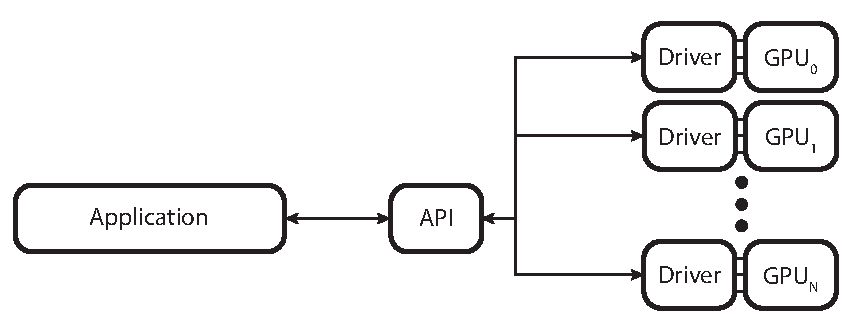
\includegraphics{Main/Images/Application_API_Driver_Overview.png}
    \label{fig:AppApiDriverOverview}
  \end{figure}

  \section{High Level Graphics Workflow}
    \todo[inline]{General overview of the stages several resources (vertices, textures, etc.) have to go through}

  \section{Motivation for a new Graphics API}
    \todo[inline]{Basically write why Vulkan is needed.}

    Traditional graphics \acrshort{api}s on Desktop systems provide high level functionality for working with a \acrshort{gpu}. In the early days, graphics hardware was used with what is called the ``fixed function pipeline'', which is basically a driver-managed state the programmer could manipulate.

  \section{The Vulkan Graphics System}
    \todo[inline]{What does it do. Where does it come from. What are people expecting from it. Cross-platform nature (in comparison maybe to PS4's libGNM made specifically for PS4 hardware).}

    \lipsum

    \subsection{Vulkan Competitors}
      \todo[inline]{OpenGL, Direct3D11, Direct3D12, libGNM (PS4)}

      \lipsum

  \section{Document Structure}
    \todo[inline]{The structure and content of this document.}

    \lipsum
